%% -*- Mode:LaTeX -*-

\chapterpreamble{0.6\textwidth}{Ingmar Bergman}{%
  Before, fortunately, I am by nature an autodidact, one who can teach himself---though it's an
  uncomfortable thing at times. Self-taught people sometimes cling too much to the technical side,
  the sure side and place technical perfection too high.
}

\chapter{How to \ldots}
\label{app:how-to}

\section{Write a Technical Text}
\label{app:how-to:write+a+technical+text}

\begin{itemize}
\item \citetitle{Booth:CR:2008} \autocite{Booth:CR:2008}
\end{itemize}
\par

\section{Citations}
\label{app:how-to:citations}

Single author:
\begin{itemize}
\item \verb!\autocite{Nicodemus:DREOS:1965}!: \autocite{Nicodemus:DREOS:1965}
\item \verb!\citetitle{Nicodemus:DREOS:1965}!: \citetitle{Nicodemus:DREOS:1965}
\item \verb!\citeauthor{Nicodemus:DREOS:1965}!: \citeauthor{Nicodemus:DREOS:1965}
\item \verb!\citeyear{Nicodemus:DREOS:1965}!: \citeyear{Nicodemus:DREOS:1965}
\end{itemize}
Multiple authors:
\begin{itemize}
\item \verb!\autocite{Sutherland:CTHSA:1974}!: \autocite{Sutherland:CTHSA:1974}
\item \verb!\citetitle{Sutherland:CTHSA:1974}!: \citetitle{Sutherland:CTHSA:1974}
\item \verb!\citeauthor{Sutherland:CTHSA:1974}!: \citeauthor{Sutherland:CTHSA:1974}
\item \verb!\citeyear{Sutherland:CTHSA:1974}!: \citeyear{Sutherland:CTHSA:1974}
\end{itemize}
\par

\section{Figures}
\label{app:how-to:figures}

\begin{figure}
  \centering
  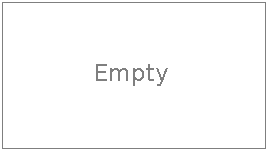
\includegraphics[draft=false,width=0.75\linewidth]{figures/empty_lscape}
  \caption[A single landscape figure]{A single landscape figure.}
  \label{fig:how-to:figures:lscape}
\end{figure}
Figure~\ref{fig:how-to:figures:lscape} contains a single image in landscape format scaled to 75\% of
the current line width.
\begin{figure}
  \centering
  \subfloat[][]{%
    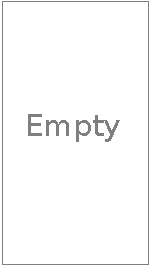
\includegraphics[draft=false,width=0.375\linewidth]{figures/empty_portrait}
    \label{fig:how-to:figures:portait:a}
  }
  \subfloat[][]{%
    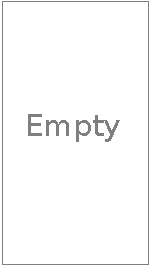
\includegraphics[draft=false,width=0.375\linewidth]{figures/empty_portrait}
    \label{fig:how-to:figures:portait:b}
  }
  \caption[A single portrait figure]{A single figure containing sub-figures
    (\protect\subref{fig:how-to:figures:portait:a} and
    \protect\subref{fig:how-to:figures:portait:b})\@.}
  \label{fig:how-to:figures:portait}
\end{figure}
Figures~\ref{fig:how-to:figures:portait:a} and \ref{fig:how-to:figures:portait:b} are sub-figures
withing figure~\ref{fig:how-to:figures:portait} but can be individually referred
to. Figures~\ref{fig:how-to:figures:portait:a} and \ref{fig:how-to:figures:portait:b} are both
scaled to 37.5\% of the current line width.
\par

\section{Tables}
\label{app:how-to:tables}

\begin{table}
  \centering
  \sffamily
  \begin{tabular}{lccr}
    \toprule
    Left aligned  & Centered & Centered & Right aligned\\
    \midrule
    \ldots & \ldots   & \ldots   & \ldots \\
    \ldots & \ldots   & \ldots   & \ldots \\
    \ldots & \ldots   & \ldots   & \ldots \\
    \bottomrule
  \end{tabular}
  \caption[A simple table]{A simple table.}
  \label{tab:how-to:tables:example1}
\end{table}
\begin{table}
  \centering
  \sffamily
  \rowcolors{3}{gray!15}{}
  \begin{tabular}{lcccr}
    \toprule
    \mrow{2}{*}{Left aligned} & \mcol{2}{c}{Centered} & \mcol{2}{c}{Centered \& Right aligned} \\
                                \cmidrule(lr){2-3}       \cmidrule(l){4-5}
                              & A & B                 & C & D\\
    \midrule
    \ldots & \ldots   & \ldots   & \ldots   & \ldots \\
    \ldots & \ldots   & \ldots   & \ldots   & \ldots \\
    \ldots & \ldots   & \ldots   & \ldots   & \ldots \\
    \bottomrule
  \end{tabular}
  \caption[Alternating row-color table]{A table with alternating row colors.}
  \label{tab:how-to:tables:example2}
\end{table}
\kant[42]
\par

\section{Source-Code Listings}
\label{app:how-to:source+code+listings}

\lstset{
  basicstyle=\small\ttfamily,
  frame=single,
}

\begin{multicols}{2}
\begin{lstlisting}[language=c++11,caption={A C++ source-code fragment, declaration},label={lst:how-to:source+code+listings:cpp+declaration}]
#include <vector>

class T {

public:

  void swap(T&);
  T& operator=(T& const);

private:

  signed           v1_;
  float[16]        v2_;
  std::vector<int> v3_;

};


// "poor man's" vertical fill
\end{lstlisting}
\vfill
\begin{lstlisting}[language=c++11,caption={A C++ source-code fragment, definition},label={lst:how-to:source+code+listings:cpp+definition}]
#include <algortihm>

void
T::swap(T& a)
{
  std::swap       (v1_, a.v1_);
  std::swap_ranges(v2_, a.v2_);
  std::swap_ranges(v3_, a.v3_);
}

T&
T::operator=(T& const rhs)
{
  T tmp(rhs);

  swap(tmp);

  return *this;
}
\end{lstlisting}
\end{multicols}
Note that listings \ref{lst:how-to:source+code+listings:cpp+declaration} and
\ref{lst:how-to:source+code+listings:cpp+definition} are {\em paired} in a twocolumn setup, to allow
easy comparison; see the \LaTeX\ source for how this is achieved.
\par

\begin{lstlisting}[language=glsl,caption={A GLSL source-code fragment}]
#version 430 core

in vec4 position;
in vec4 normal;
in vec2 tcoords;

out vp_out_t {
       vec3  position_wc;
       vec3  normal_wc;
       vec2  tcoords;
  flat int   mtl_id;
} vp_out;

void
main()
{
  // this 'drives' the rasterizer; p' = mvp * p
  gl_Position         = xform_projection;
  gl_Position        *= xform_view;
  gl_Position        *= xform_model;
  gl_Position        *= position;

  // these will be interpolated and used in the fragment program
  // note: position/normal stay in world coordinates!
  vp_out.position_wc = (xform_model * position).xyz;
  vp_out.normal_wc   = normalize(transpose(inverse(xform_model)) *
                       normal).xyz;
  vp_out.tcoords     = tcoords;
  vp_out.mtl_id      = material_id;
}
\end{lstlisting}
\begin{lstlisting}[language=hlsl,caption={A HLS source-code fragment}]
/* uniform */ StructuredBuffer<light> light_list;
/* uniform */ lambert_material        material;

fp_output
fp_main(fp_input input)
{
  fp_output result;

  float4 ambient  = color_black;
  float4 diffuse  = color_black;
  float4 specular = color_black;

  accumulate_lights(/* in */    light_list, input.position.xyz,
                    /* in */    normalize(input.normal.xyz),
                    /* in */    viewer_position.xyz,
                    /* in */    material.shininess,
                    /* inout */ ambient, diffuse, specular);

  result.color    =            material.emission;
  result.color   += ambient  * material.ambient;
  result.color   += diffuse  * material.diffuse;
  result.color   += specular * material.specular;
  result.color.a  = material.diffuse.a;

  return result;
}
\end{lstlisting}
\par

\section{Miscellaneous}
\label{app:how-to:miscellaneous}

\ldots
\par

%%% Local Variables:
%%% mode: latex
%%% TeX-master: "../main"
%%% End:
